\documentclass[11pt, letterpaper]{memoir}
\usepackage{HomeworkStyle}
\geometry{margin=0.75in}



\begin{document}

	\begin{center}
		{\large Quiz 11.2 -- Rotational Spectroscopy}
	\end{center}
	{\large Name: \rule[-1mm]{4in}{.1pt} 

\subsection*{}
Below is a microwave spectrum of the CN radical

\noindent
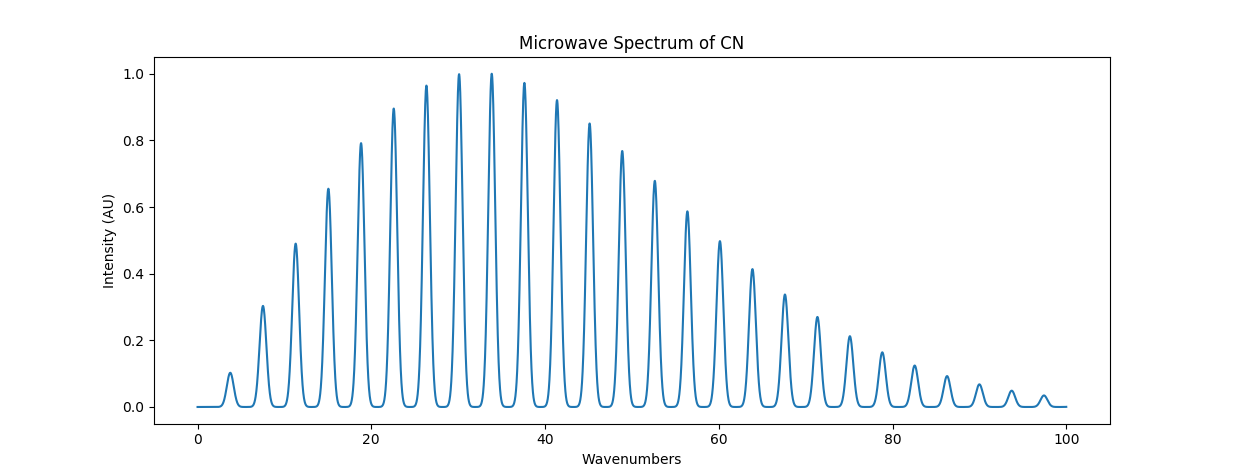
\includegraphics[trim= 0 0 0 0, clip=true, width=\linewidth]{CN_Microwave}

\noindent
Using the spectrum, find the following quantities:
\begin{enumerate}
	\item $\tilde{B}$
	\item $r$ (Bond length)
	\item Temperature
	\item $\tilde{D}_J$
\end{enumerate}
\end{document}
